\documentclass[tikz,border=2pt]{standalone}
\usepackage{amsmath,amssymb}
\usepackage{tikz}

\begin{document}
% The complement of A inside the universe U is everything in U that is not in A.
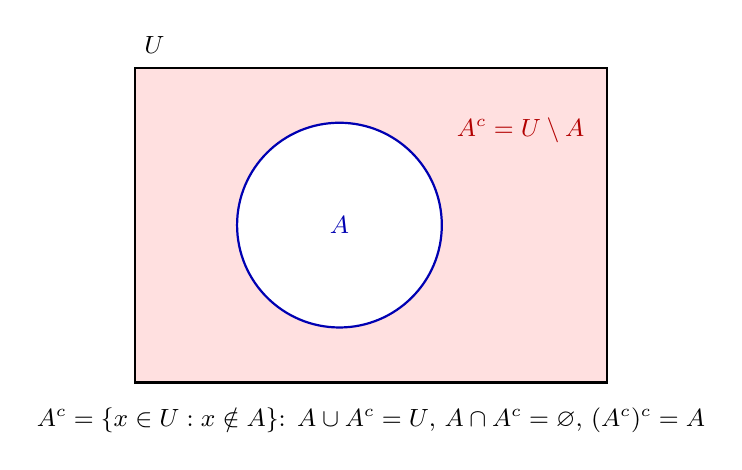
\begin{tikzpicture}[every node/.style={font=\small}]
	\fill[red!12] (-3,-2) rectangle (3,2);
	\fill[white] (-0.4,0) circle (1.3);
	\draw[thick] (-3,-2) rectangle (3,2);
	\draw[thick, blue!70!black] (-0.4,0) circle (1.3);
	\node[blue!70!black] at (-0.4,0) {$A$};
	\node[red!70!black] at (1.9,1.2) {$A^{c}=U\setminus A$};
	\node[anchor=south west] at (-3,2.05) {$U$};
	\node[anchor=north, align=center] at (0,-2.2) {$A^{c}=\{x\in U: x\notin A\}$: $A\cup A^{c}=U$, $A\cap A^{c}=\varnothing$, $(A^{c})^{c}=A$};
\end{tikzpicture}
\end{document}
